\documentclass[12pt,reqno,oneside,hidelinks]{article}
% \documentclass[12pt, final]{siamonline171218}
% \usepackage[pdfborder={0 0 0.5 [3 2]}]{hyperref}%
\usepackage[left=0.85in,right=0.85in,top=0.75in,bottom=1in]{geometry}%
\usepackage{amsmath}
\usepackage{amssymb}
\usepackage{amsthm}
\usepackage{graphicx}
\usepackage{enumerate}
\usepackage{float}
\usepackage{bm}
\usepackage[stable]{footmisc}

\usepackage{packages}
\usepackage{wrapfig}
\usepackage{subfigure}
\usepackage[font=footnotesize]{caption}

% \newtheorem{theorem}{Theorem}
% \newtheorem{lemma}[theorem]{Lemma}
% \newtheorem{corollary}{Corollary}

% \theoremstyle{definition}
% \newtheorem{definition}[theorem]{Definition}

% \theoremstyle{remark}
% \newtheorem{remark}[theorem]{Remark}

\def\noi{\noindent}
\def\T{{\mathbb T}}
\def\R{{\mathbb R}}
\def\N{{\mathbb N}}
\def\Z{{\mathbb Z}}
\def\C{{\mathbb C}}
\def\Q{\mathbb{Q}}

\newcommand{\vK}{\bm{\mathit{K}}}
\newcommand{\calP}{\mathcal{P}}
\newcommand{\calA}{\mathcal{A}}

\setlength{\parindent}{0em}
\setlength{\parskip}{1em}
\renewcommand{\baselinestretch}{1.1}

\title{Research Statement}
\date{\vspace{-12ex}}

\begin{document}

\thispagestyle{empty}

\section*{Research statement}

My main research focus is on coherent structures in dynamical systems. Dynamical systems are mathematical models which evolve in time. A prototypical example is a model of a swinging pendulum, which can be expressed as an ordinary differential equation (ODE) describing the evolution of the angular position and angular velocity of the pendulum. The dynamical systems I study are nonlinear wave equations, which are typically expressed mathematically as partial differential equations (PDEs). These equations describe the time evolution of a function representing a wave profile. In particular, I study coherent structures in Hamiltonian systems. 
Hamiltonian systems are characterized by a conserved quantity, such as energy, that remains constant in time. Coherent structures are spatial patterns which maintain their shape as the system evolves in time. Examples of coherent structures include solitary waves, which are localized disturbances that maintain their shape as they propagate at a constant velocity; wavetrains, which are periodic disturbances that also propagate at a constant velocity; and breathers, which are disturbances which are localized in space but oscillate in time. Solitary waves have been a topic of interest since the 19th century, when John Scott Russell observed a single, large surface wave on the Edinburgh-Glasgow Union Canal in Scotland which propagated along the canal undisturbed for a few miles before eventually decaying. This phenomenon was explained mathematically by the Korteweg–De Vries (KdV) equation 
\[
u_t + u_{xxx} + 6 u u_x = 0,
\]
which has both solitary wave and wavetrain solutions.
\begin{figure}[H]
    \centering
    \begin{tabular}{cc}
        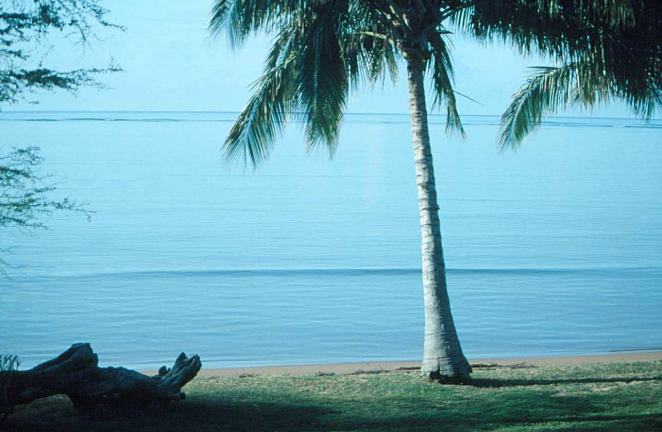
\includegraphics[width=7cm]{images/SolitaryWaveHawaii.png} &
        % 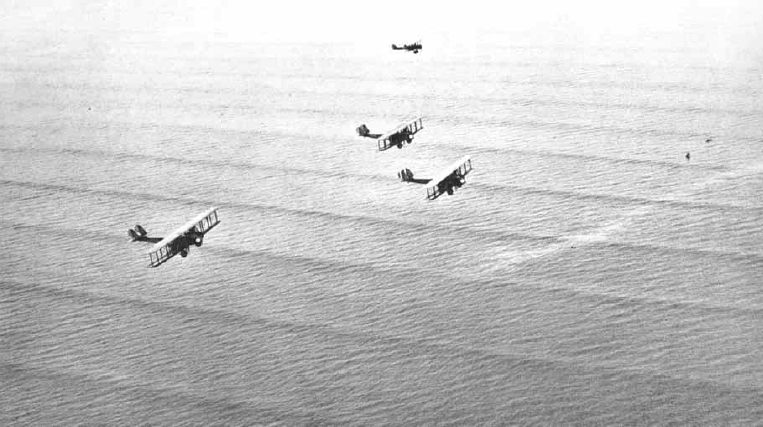
\includegraphics[width=7cm]{images/cnoidalwaves.png} 
        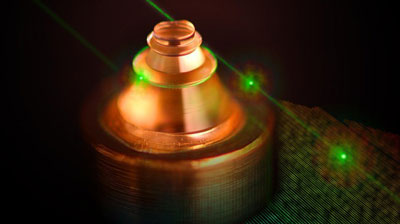
\includegraphics[width=8.1cm]{images/resonator.jpg} 
        % 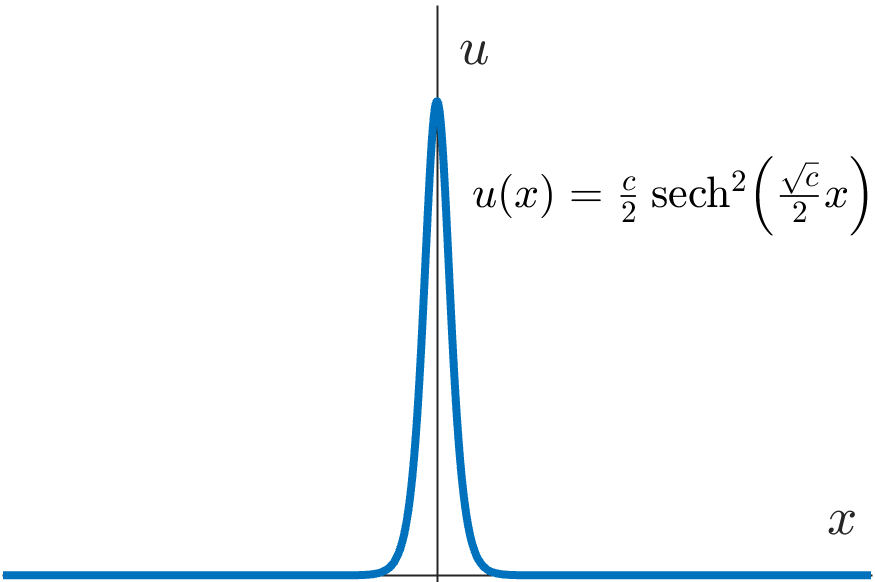
\includegraphics[width=7cm]{images/kdvsoliton.png} &
        % 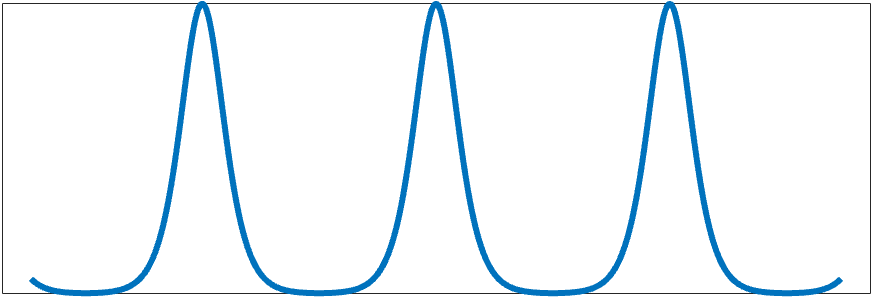
\includegraphics[width=7cm]{images/kdvcn.png}      
    \end{tabular}
    \caption{Solitary wave off the coast of Hawaii \cite{Andriopoulos2009} (left). Optical solitons in a microresonator \cite{MarinPalomo2017} (right) }
    \label{fig:solitarywaves}
\end{figure}
Although solitary waves were originally discovered as a water wave phenomenon, they have applications in many fields such as fiber optics, plasma physics, quantum mechanics, molecular biology, and neuroscience (\cref{fig:solitarywaves}). More generally, many nonlinear, dispersive PDEs exhibit solitary wave solutions. My research falls into two broad categories: multi-pulse solitary waves in Hamiltonian systems, and coherent structures in optical lattices. 

\section*{Multi-pulse solitary waves in Hamiltonian systems}

The prototypical nonlinear wave equation has a primary solitary wave solution, also known as a pulse solution, which looks like a single localized ``bump'' (\cref{fig:kdvpp}, left). In many systems, multi-pulse solutions also exist; these are ``multi-bump'' solitary waves which resembles multiple, well separated copies of the primary pulse solution. (Notably, multi-pulse solutions do not exist to the KdV equation). 
The entire multi-pulse travels as a unit and maintains its shape unless perturbed. In addition to having applications in nonlinear optics and neuroscience \cite{Evans1982}, multi-pulses are interesting mathematically. In my research, I explore the existence and stability of these multi-pulse structures. A crucial step in this process is determining the spectrum of the linearization of the underlying system about these multi-pulse solutions. When a multi-pulse is perturbed, interactions between the individual pulses in the structure are revealed, which are a consequence of the inherent nonlinearity of the system. The dynamics of these interactions are determined by the eigenvalues of the linearized system and their corresponding eigenfunctions.

\begin{figure}[H]
    \centering
    \begin{tabular}{cc}
        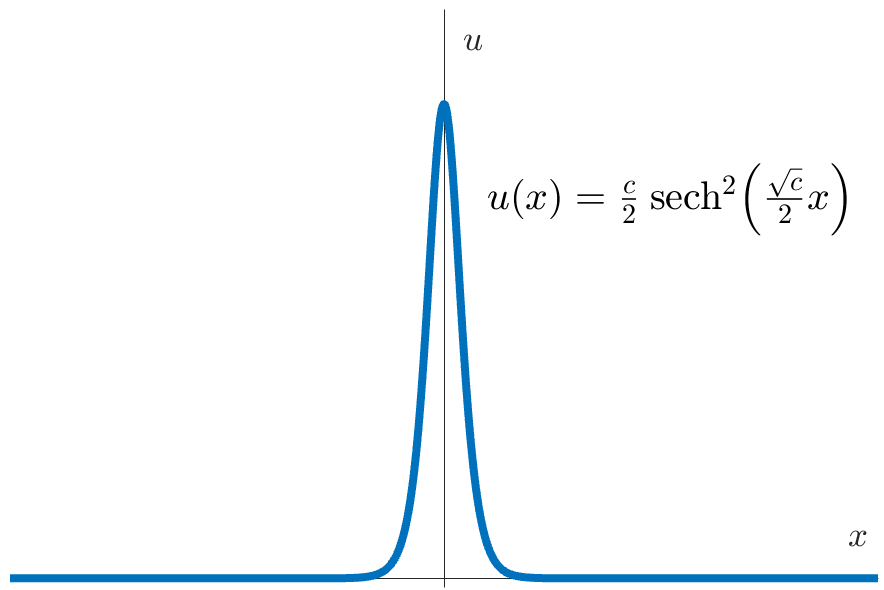
\includegraphics[width=6cm]{images/KdVsolitoneq.png} &
        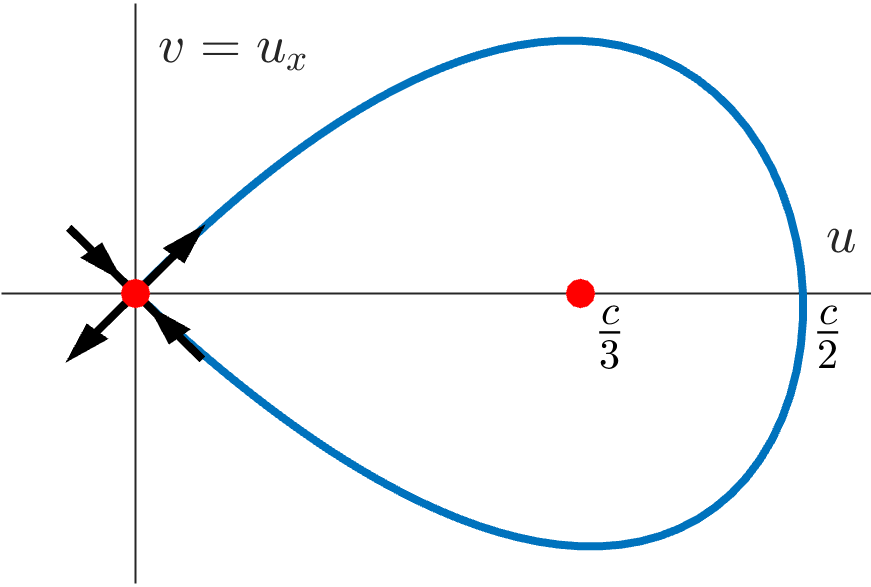
\includegraphics[width=6cm]{images/KdVphaseportait.png} 
    \end{tabular}
    \caption{Primary solitary wave solution $u(x)$ to the KdV equation. Left panel is plot of $u$ vs $x$. Right panel is plot of $u_x$ vs $u$, showing solitary wave as a homoclinic orbit. }
    \label{fig:kdvpp}
\end{figure}

My primary mathematical approach comes from spatial dynamics. From this viewpoint, a solitary wave $u(x)$ is a homoclinic orbit evolving in the spatial variable $x$. For example, the solitary wave solution $u(x)$ to the KdV equation which moves with constant speed $c$ (\cref{fig:kdvpp}, left panel) is a solution to the second order ODE $u_{xx} + 3 u^2 - c u = 0$. This can be written as the two-dimensional dynamical system 
\[
\frac{d}{dx}\begin{pmatrix}u\\v\end{pmatrix}
= \begin{pmatrix}v \\ cu - 3u^2\end{pmatrix}
\]
by taking $v = u_x$. From this perspective, the solitary wave solution $(u(x), v(x))$ is a homoclinic orbit connecting the unstable and stable manifolds of the saddle equilibrium at the origin (\cref{fig:kdvpp}, right panel), which represents the rest state of the system. 

Multi-pulses are multi-loop homoclinic orbits. From a theoretical standpoint, multi-pulses can be constructed using Lin's method \cite{Lin2008}, a version of the Lyapunov-Schmidt method used to find solutions which remain near a homoclinic orbit. Heuristically, this process involves ``gluing together'' multiple copies of the primary pulse solution end-to-end using small remainder functions (\cref{fig:linsmethod}). Lin's method can also be used to construct periodic orbits and multi-loop periodic orbits. Construction of multi-pulse solutions is constrained by the geometry of the primary pulse and the underlying system. In \cref{fig:linsmethod}, for example, multi-pulses only exist when the tail oscillations of the individual pulses match up. Once a multi-pulse has been constructed, the next step is to analyze its stability.

\begin{figure}
    \centering
    \begin{tabular}{cc}
        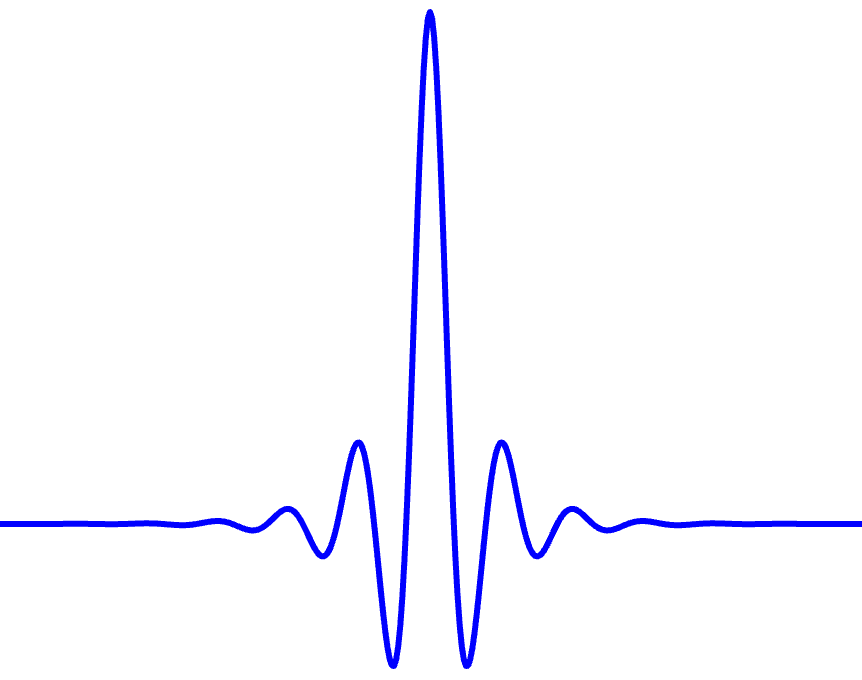
\includegraphics[width=6cm]{images/linchen1.png} &
        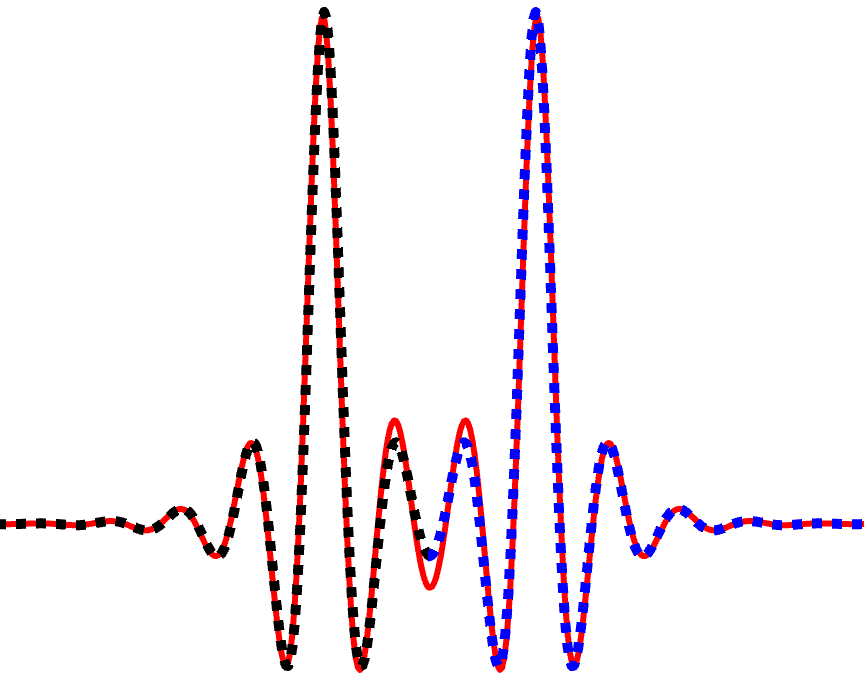
\includegraphics[width=6cm]{images/linchen2.png} 
    \end{tabular}
    \caption{Cartoon illustrating construction of a double pulse solution using Lin's method. Left panel shows primary pulse solution. Right panel shows two copies of the primary pulse solution (black and blue dotted lines) placed end-to-end. Double pulse solution (red solid line) is close, but not equal, to this.}
    \label{fig:linsmethod}
\end{figure}

\begin{wrapfigure}[8]{R}{6cm}
    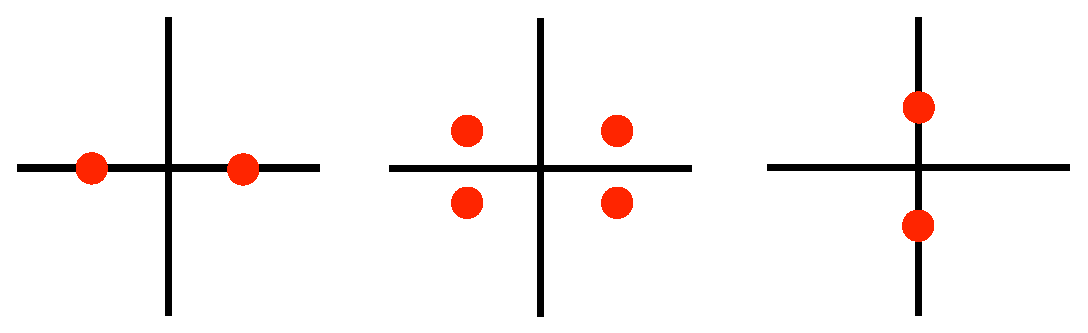
\includegraphics[width=6cm]{images/inteigpattern.eps}
    \caption{Possible interaction eigenvalue patterns in a Hamiltonian system.} 
    \label{fig:inteigpattern}
\end{wrapfigure}
The first step in this process is to compute the spectrum of the linearization of the underlying system about the multi-pulse solution. In general, each pulse that is added to a multi-pulse structure is associated with one or more eigenvalues in the spectrum \cite{Sandstede1998}. I refer to these as interaction eigenvalues, since they result from nonlinear interactions between the tails of neighboring pulses. The systems I study are Hamiltonian, which are not covered by the results of \cite{Sandstede1998}. On one hand, the Hamiltonian structure is very helpful, since all eigenvalues must come in quartets of the form $\pm \alpha \pm \beta i$. This means that each additional set of interaction eigenvalues must occur in one of the three patterns in \cref{fig:inteigpattern}. On the other hand, the presence of any eigenvalue with nonzero real part implies that there is an unstable eigenvalue. This means that Hamiltonian systems cannot be dissipative, which makes stability analysis more difficult. My main results relate the spectral pattern of the interaction eigenvalues to the underlying geometry of the multi-pulse. In all cases, the spectral pattern is determined by this geometry. 

In addition to theoretical work, I make extensive use of numerical analysis, both to generate hypotheses and to verify analytical results. For multi-pulses, I start by constructing the primary solitary wave, which either involves parameter continuation from a known solution using the software package AUTO or an energy minimization method such as the string method \cite{Chamard2011} or the mountain pass method \cite{Chen1997}. I then glue together multiple copies of the primary solitary wave and use a root-finding method such as conjugate gradient to construct a multi-pulse. I compute the spectrum using an eigenvalue solver on an appropriate discretization of the linearized system.

\subsection*{Discrete nonlinear Schr\"odinger equation}

The discrete nonlinear Schr{\"o}dinger equation (DNLS) 
\begin{align*}
    i \frac{d}{dt} u_n + d(u_{n+1} - 2 u_n + u_{n-1}) + |u_n|^2 u_n && n \in \mathbb{Z}
\end{align*}
is the discrete analogue to the nonlinear Schr{\"o}dinger equation (NLS) on the integer lattice. The parameter $d$ quantifies the degree of coupling between adjacent lattice sites. In addition to being a fundamental model of a nonlinear dynamical system on a lattice, DNLS has applications to nonlinear optics and condensed matter physics \cite{Kevrekidis2009}. For all values of $d$, DNLS has a stable, primary pulse solution (\cref{fig:DNLS2p}, left panel). Provided that the individual peaks are separated by a sufficiently large number of lattice points, I use Lin's method to prove that multi-pulse solutions exist as long as the following geometric constraint is satisfied: neighboring peaks must either be out-of-phase or in-phase \cite{Parker2020}. Furthermore, I prove this geometry determines the stability of multi-pulses. For double pulses, the in-phase double pulse is unstable, since there is eigenvalue with positive real part, and the out-of-phase double pulse is neutrally stable, since the entire spectrum lies on the imaginary axis (see \cref{fig:DNLS2p}). For general multi-pulses, the entire structure is unstable if any pair of neighboring peaks are in-phase. The only neutrally stable multi-pulses are those in which every pair of neighboring peaks is out-of-phase. The proof of this result \cite[Theorem 2]{Parker2020} adapts the method of \cite{Sandstede1998} to the Hamiltonian case, and uses Lin's method to construct the eigenfunctions corresponding to the interaction eigenvalues. This reduces the spectral problem for an $n$-pulse to finding the eigenvalues of an $n\times n$ matrix.

\begin{figure}
    \centering
    \begin{tabular}{ccc}
        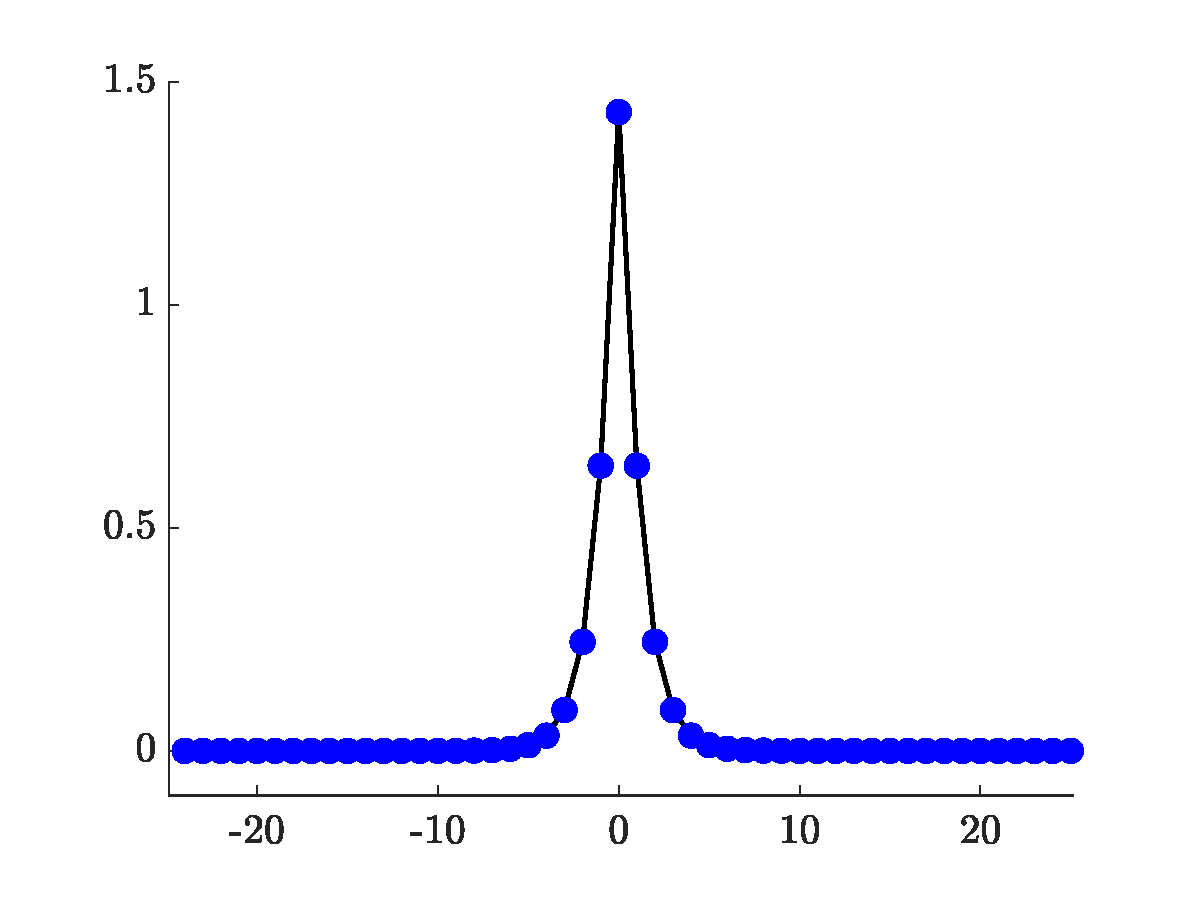
\includegraphics[width=5cm]{images/DNLSprimary.eps} &
        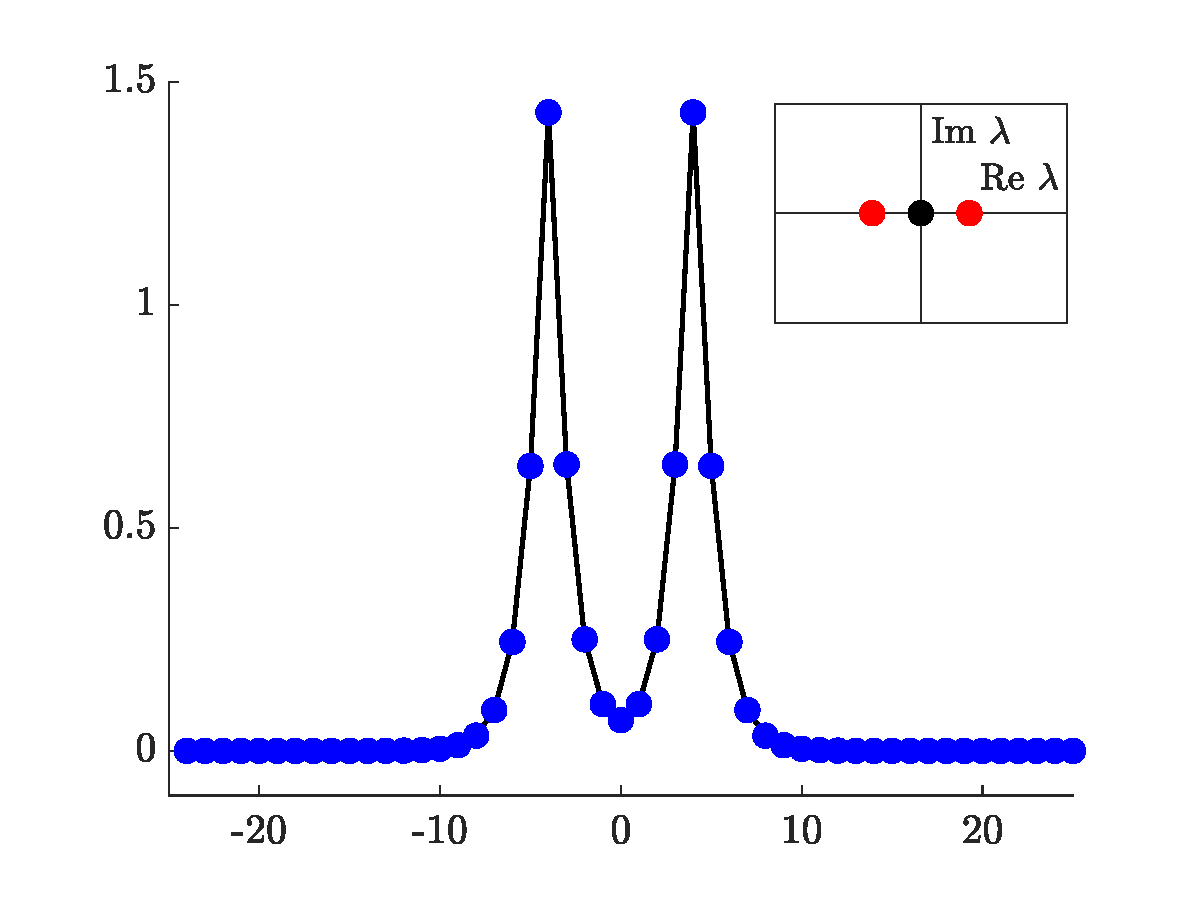
\includegraphics[width=5cm]{images/DNLSunstable2p.eps} &
        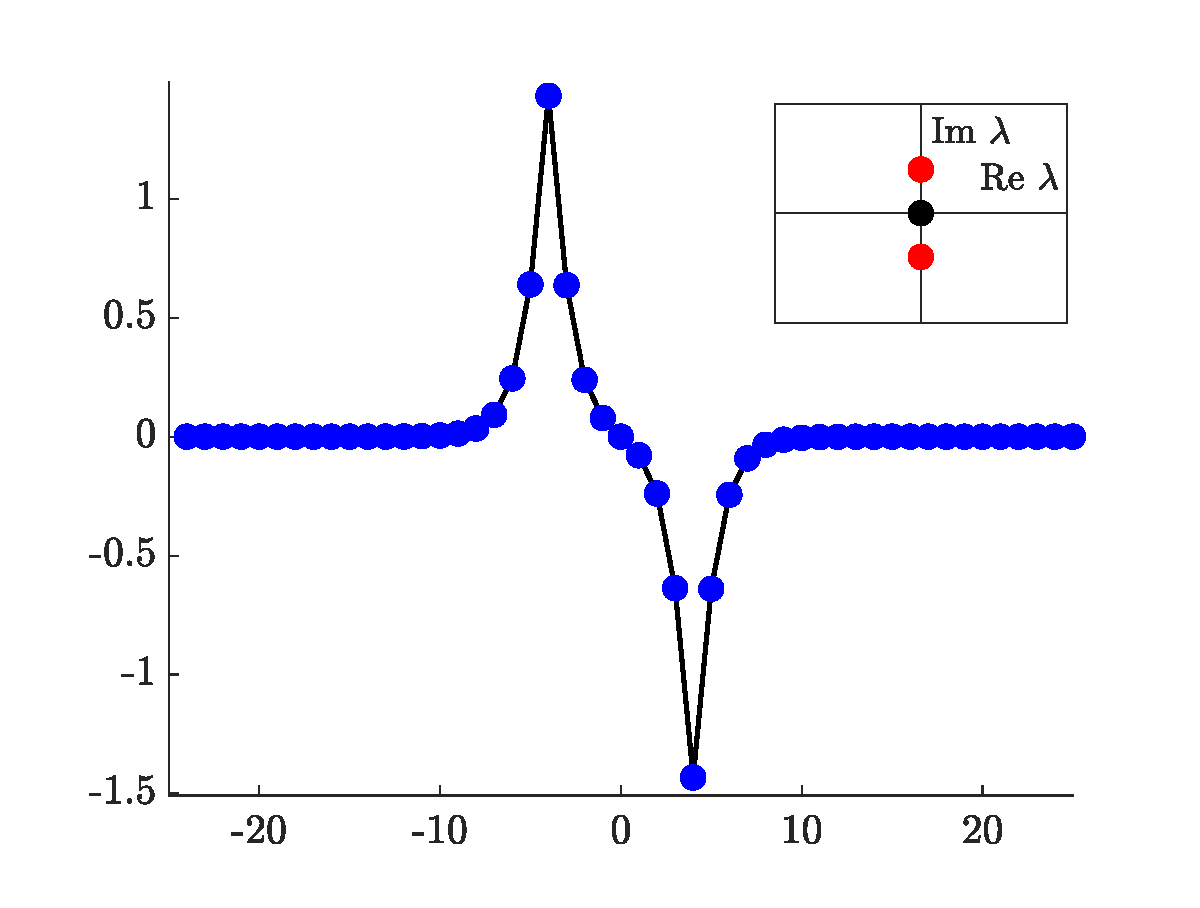
\includegraphics[width=5cm]{images/DNLSstable2p.eps} 
    \end{tabular}
    \caption{Primary pulse solution for DNLS (left). Out-of-phase (middle) and in-phase (right) double pulse solutions for DNLS. Interaction eigenvalue patterns for double pulses are shown in insets. Black dot is a kernel eigenvalue with algebraic multiplicity 2.}
    \label{fig:DNLS2p}
\end{figure}


\subsection*{Chen-McKenna suspension bridge equation}

The Chen-McKenna suspension bridge equation 
\begin{align*}
    u_{tt} + u_{xxxx} + \mathrm{e}^{u-1} - 1 &= 0 
\end{align*}
is a smooth approximation to a model for waves propagating on an infinitely long suspended beam, and is motivated by observations of traveling waves on suspension bridges \cite{McKenna1990,Chen1997}. For wave speeds $c$ between 0 and $\sqrt{2}$, a primary solitary wave solution exists \cite{Berg2018}, which has exponentially decaying, oscillatory tails (\cref{fig:chen2p}, top left). Provided that the individual peaks are sufficiently well separated, multi-pulse solutions again exist as long as the following geometric constraint is satisfied: the tail oscillations of neighboring peaks must overlap in-phase (see the cartoon illustration in \cref{fig:linsmethod}). This constraint is a consequence of the specific alignment of the unstable and stable manifolds which is necessary for a multi-loop homoclinic orbit to be possible. As a result, the distance between consecutive peaks is, to leading order, an integer multiple of a phase parameter. This is illustrated in the top right panel of \cref{fig:chen2p}, which plots the first four double pulse solutions on the same graph. As with DNLS, the stability of multi-pulses depends on their geometry. Double pulses, for example, alternate between unstable (bottom left of \cref{fig:chen2p}, corresponding to even integers) and neutrally stable (bottom right of \cref{fig:chen2p}, corresponding to odd integers). I prove these spectral results using an extension of the Krein matrix \cite{Kapitula2020}, a tool which projects the infinite-dimensional spectral problem onto a finite-dimensional space. 

\begin{figure}
    \centering
    \begin{tabular}{cc}
        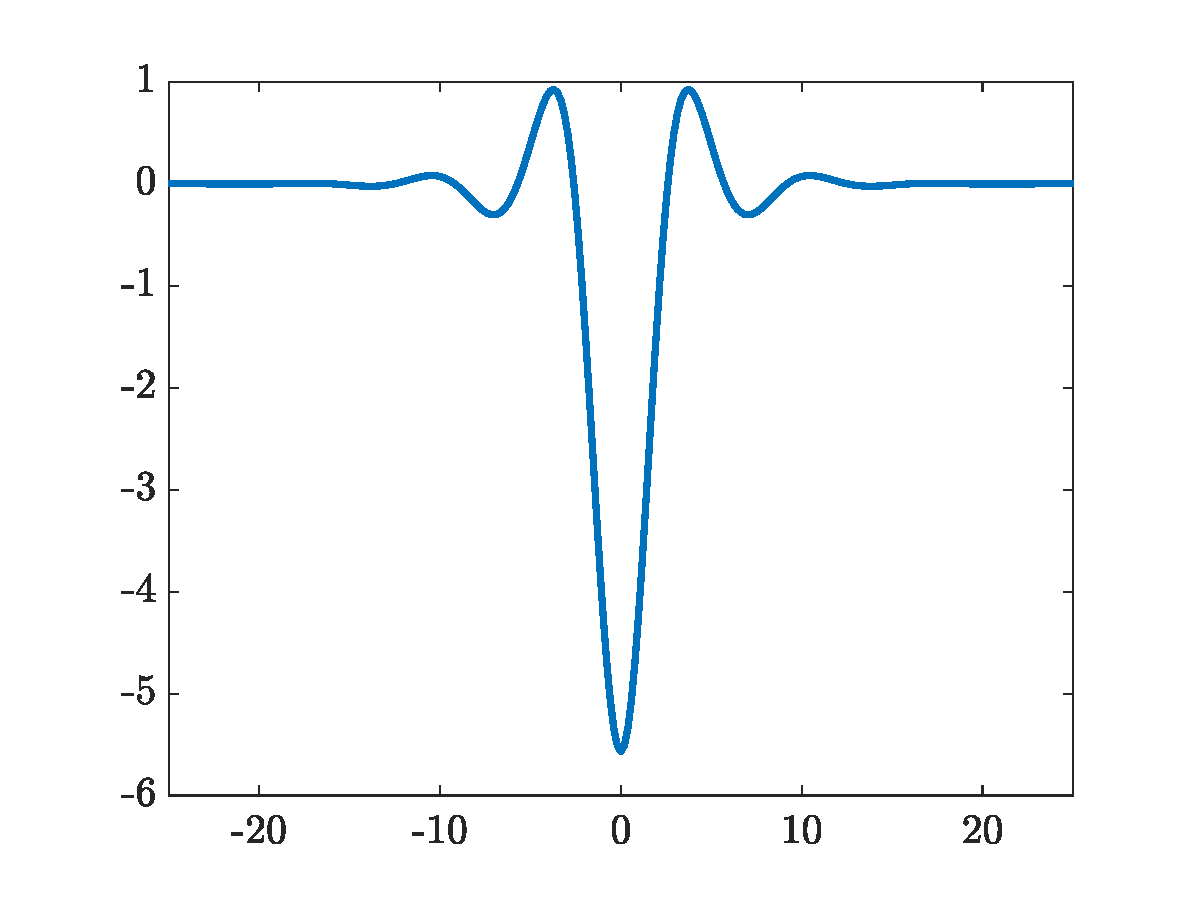
\includegraphics[width=7cm]{images/chen1p.eps} &
        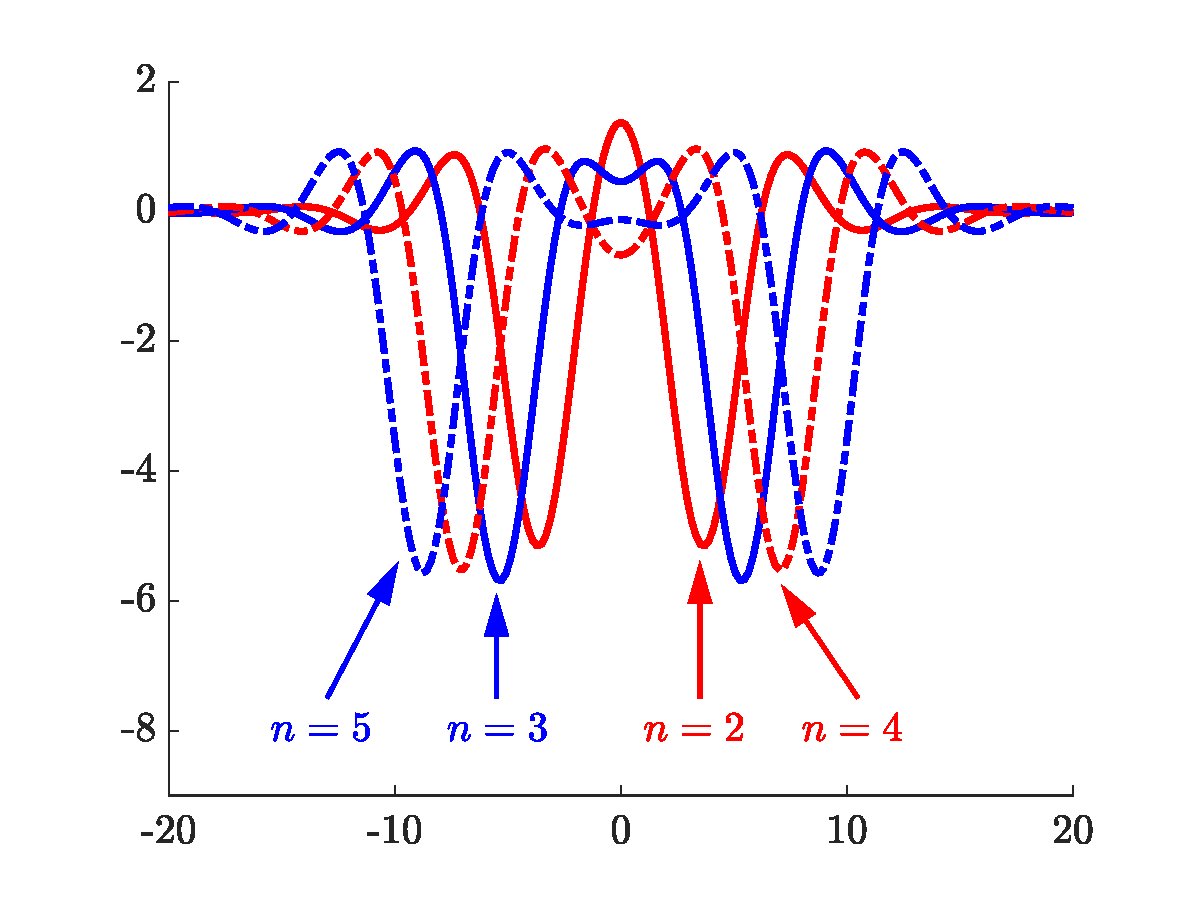
\includegraphics[width=7cm]{images/chenDPall.eps} \\
        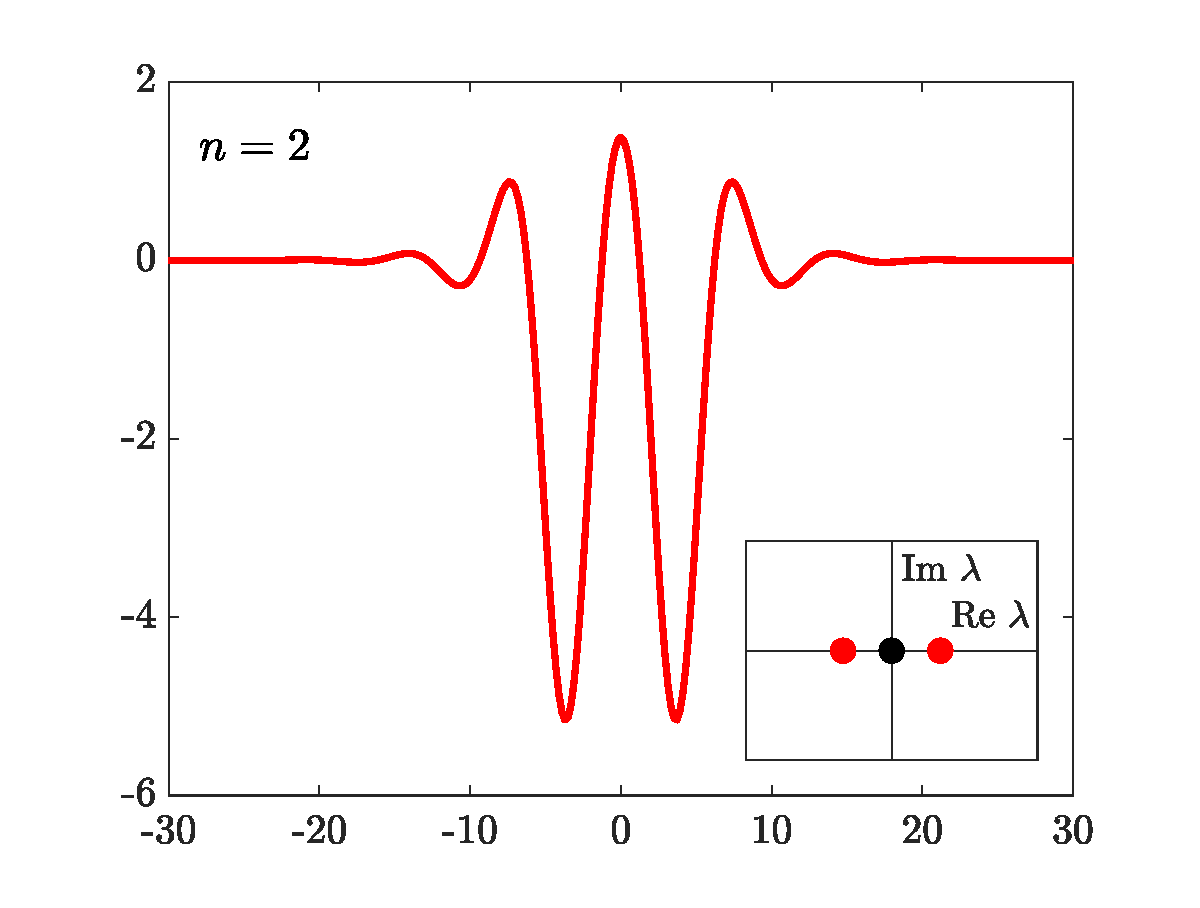
\includegraphics[width=7cm]{images/chen2punstable.eps} &
        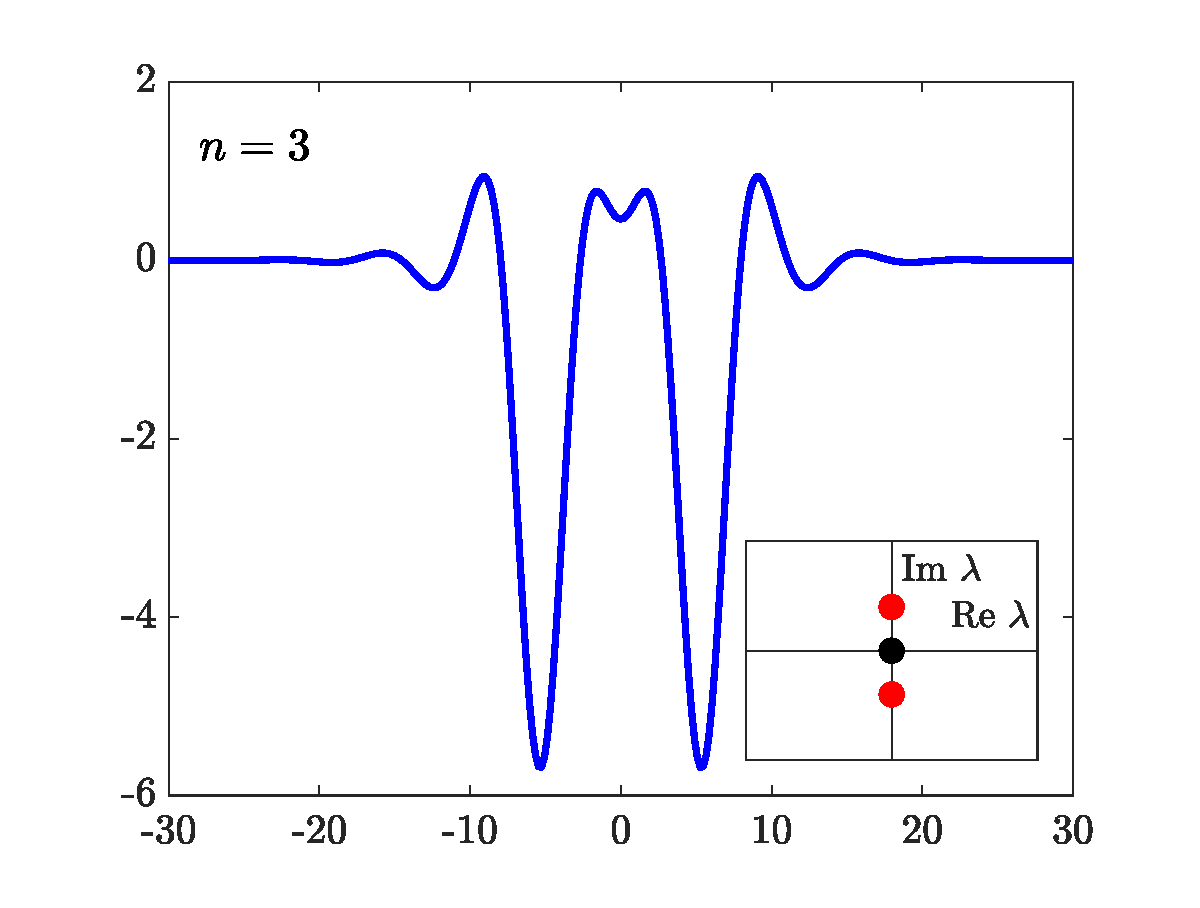
\includegraphics[width=7cm]{images/chen2pstable.eps} 
    \end{tabular}
    \caption{Primary pulse solution for Chen-Mckenna (top left). First four double pulse solutions (top right). Unstable double pulse for $n=2$ (bottom left) and neutrally stable double pulse for $n=3$ (bottom right). Interaction eigenvalue patterns for double pulses are shown in insets. Black dot is a kernel eigenvalue with algebraic multiplicity 2.}
    \label{fig:chen2p}
\end{figure}

\subsection*{Fifth order KdV equation}

The fifth-order Korteweg de-Vries equation (KdV5)
\begin{align*}
    u_t - u_{xxxxx} + u_{xxx} + 2 u u_x &= 0
\end{align*} 
is a weakly nonlinear long wave approximation to capillary-gravity wave problem which also has applications to plasma physics and laser optics \cite{Pelinovsky2007}. Multi-pulse solutions to KdV5 exist \cite{SandstedeStrut}, but their stability analysis is complicated due to the fact that the essential spectrum for all localized solutions comprises the entire imaginary axis. In particular, this means that any purely imaginary interaction eigenvalues would be embedded in the essential spectrum, which makes them difficult to locate.

To simplify the situation, I impose periodic boundary conditions on the problem and look instead at periodic multi-pulses, which are periodic orbits containing multiple peaks. From a spatial dynamics perspective, a periodic multi-pulse is a multi-loop periodic orbit which is close to the primary homoclinic orbit. A periodic double pulse, for example, is constructed by gluing two single pulses together at both ends. Since this construction involves two length parameters $X_0$ and $X_1$ (\cref{fig:periodic}, left), there is an extra degree of freedom when compared to double pulses on the real line. As a consequence, I prove that periodic double pulses exist in a continuous family, in which asymmetric periodic double pulses (those with $X_0 \neq X_1$) bifurcate from symmetric periodic double pulses (those with $X_0 = X_1$) in a series of pitchfork bifurcations (\cref{fig:periodic}, center) \cite{ParkerKdV}. The advantage of looking at periodic solutions is that the essential spectrum becomes a discrete set of eigenvalues on the imaginary axis (blue open circles in \cref{fig:periodic}, right). Purely imaginary interaction eigenvalues can then lie between essential spectrum eigenvalues, which avoids the problem of embedded eigenvalues. 

\begin{figure}
    \begin{center}
    \includegraphics[width=7cm]{images/2pulse3d.png} \hspace{-1cm}
    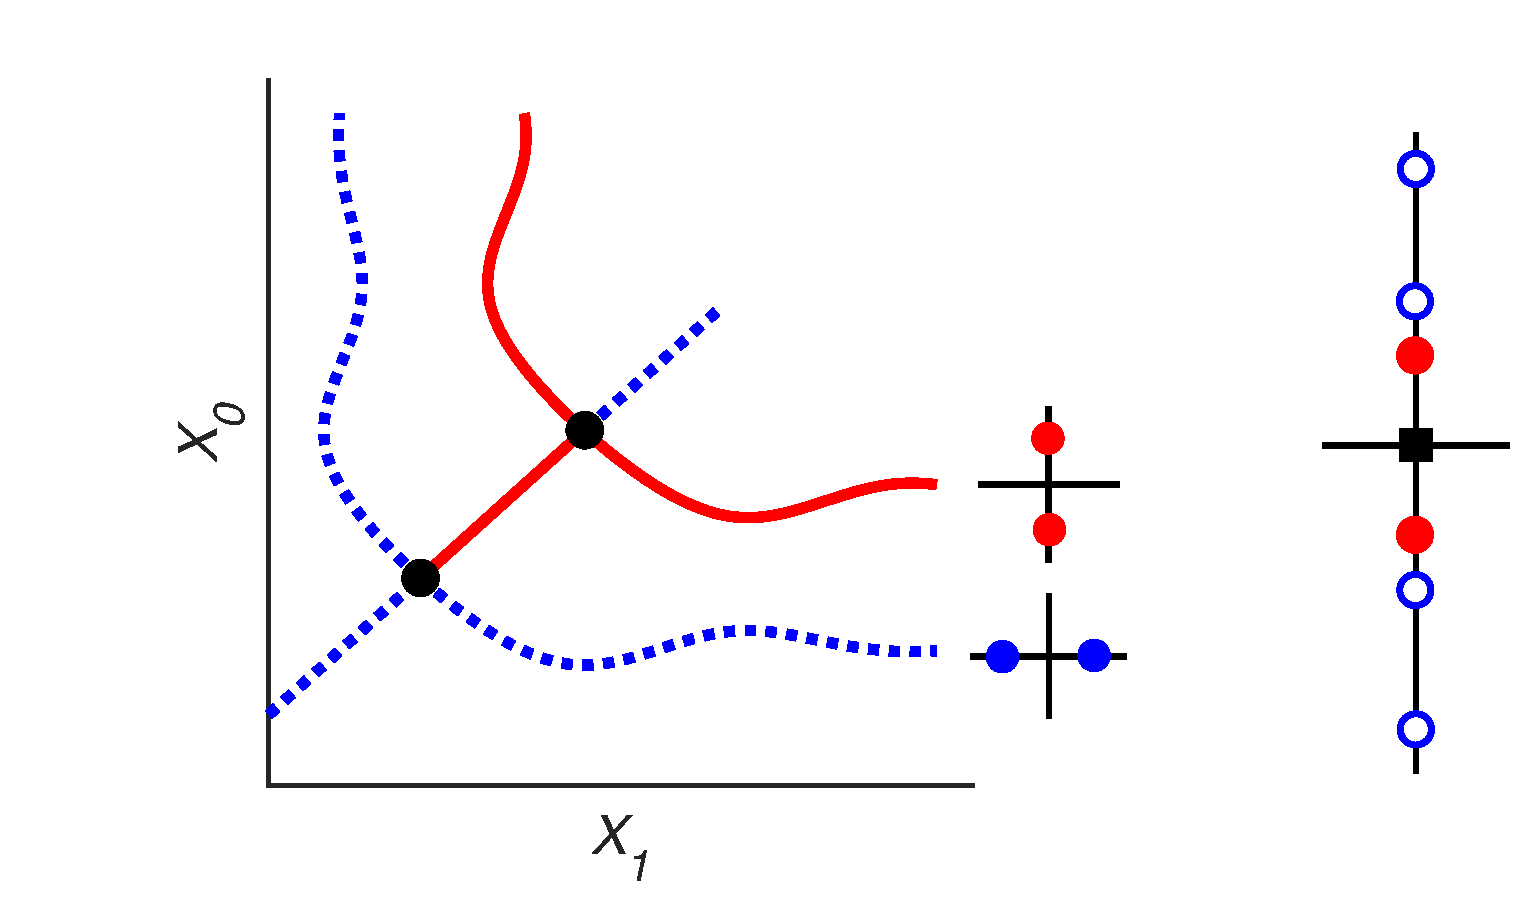
\includegraphics[width=9cm]{images/2pitchforkcoloreig2.eps}
    \end{center}
    \caption{Construction (left) and bifurcation diagram (center) of periodic double pulse solutions to KdV5. Spectrum of neutrally stable periodic double pulses (right) comprising interaction eigenvalues (red filled circles), essential spectrum eigenvalues (blue open circles), and kernel eigenvalue with algebraic multiplicity 2 (black square).}
    \label{fig:periodic}
\end{figure}
    
Using Lin's method, I prove that the eigenvalues associated with a periodic multi-pulse can be found by solving a block matrix equation \cite[Theorem 5.3]{ParkerKdV} for the eigenvalues $\lambda$. To leading order, this is given by
    \begin{equation}\label{blockmatrix}
    \det \begin{pmatrix}
    K(\lambda) - \frac{1}{2} \lambda \tilde{M} K^+(\lambda) & \lambda^2 M_c I \\
    -\frac{1}{2} \lambda M_c K^+(\lambda) & A - \lambda^2 MI  
    \end{pmatrix} = 0.
    \end{equation}
The essential spectrum eigenvalues are encoded by the matrix $K(\lambda)$, which, to leading order, only depends on the background state and size of the periodic domain; in particular, it is independent of the periodic multi-pulse solution. The interaction eigenvalues are encoded by the matrix $A$, which depends on the geometry of the periodic multi-pulse. $M$, $M_c$, and $\tilde{M}$ are fundamental constants associated with the primary pulse solution. As long as the periodic domain size is not too large, the interaction eigenvalues and essential spectrum eigenvalues do not interfere with each other. As a consequence, for a periodic double pulse, there is a pair of interaction eigenvalues which is either real or purely imaginary depending on the geometry of the periodic 2-pulse (\cref{fig:periodic}, center). The eigenvalue pattern switches between real and imaginary at the pitchfork bifurcation points.  
    
There is, however, an additional complication in the periodic case. As the periodic domain size $X$ is increased, the essential spectrum eigenvalues move towards the origin. At a critical value of $X$,  there will be a collision between one of the essential spectrum eigenvalues and a purely imaginary interaction eigenvalue. As $X$ is further increased, I prove that a brief instability bubble is formed, wherein the two eigenvalues collide, move off the imaginary axis, trace an approximate circle in the complex plane, and recombine on the imaginary axis in a ``reverse'' collision (see left panel of \cref{fig:kreinbubble1} for a cartoon) \cite{ParkerKdV}. This instability bubble, which we call a Krein bubble since the eigenvalues involved in the collision have opposite Krein signature, is a direct consequence of the block matrix reduction \cref{blockmatrix}. A numerical simulation of the Krein bubble, computed using parameter continuation with AUTO, is shown in the right panel of \cref{fig:kreinbubble1}. The location and size of the Krein bubble in the simulation agree with that predicted by the theory \cite{ParkerKdV}.
    
\begin{figure}
\begin{center}
\begin{tabular}{cc}
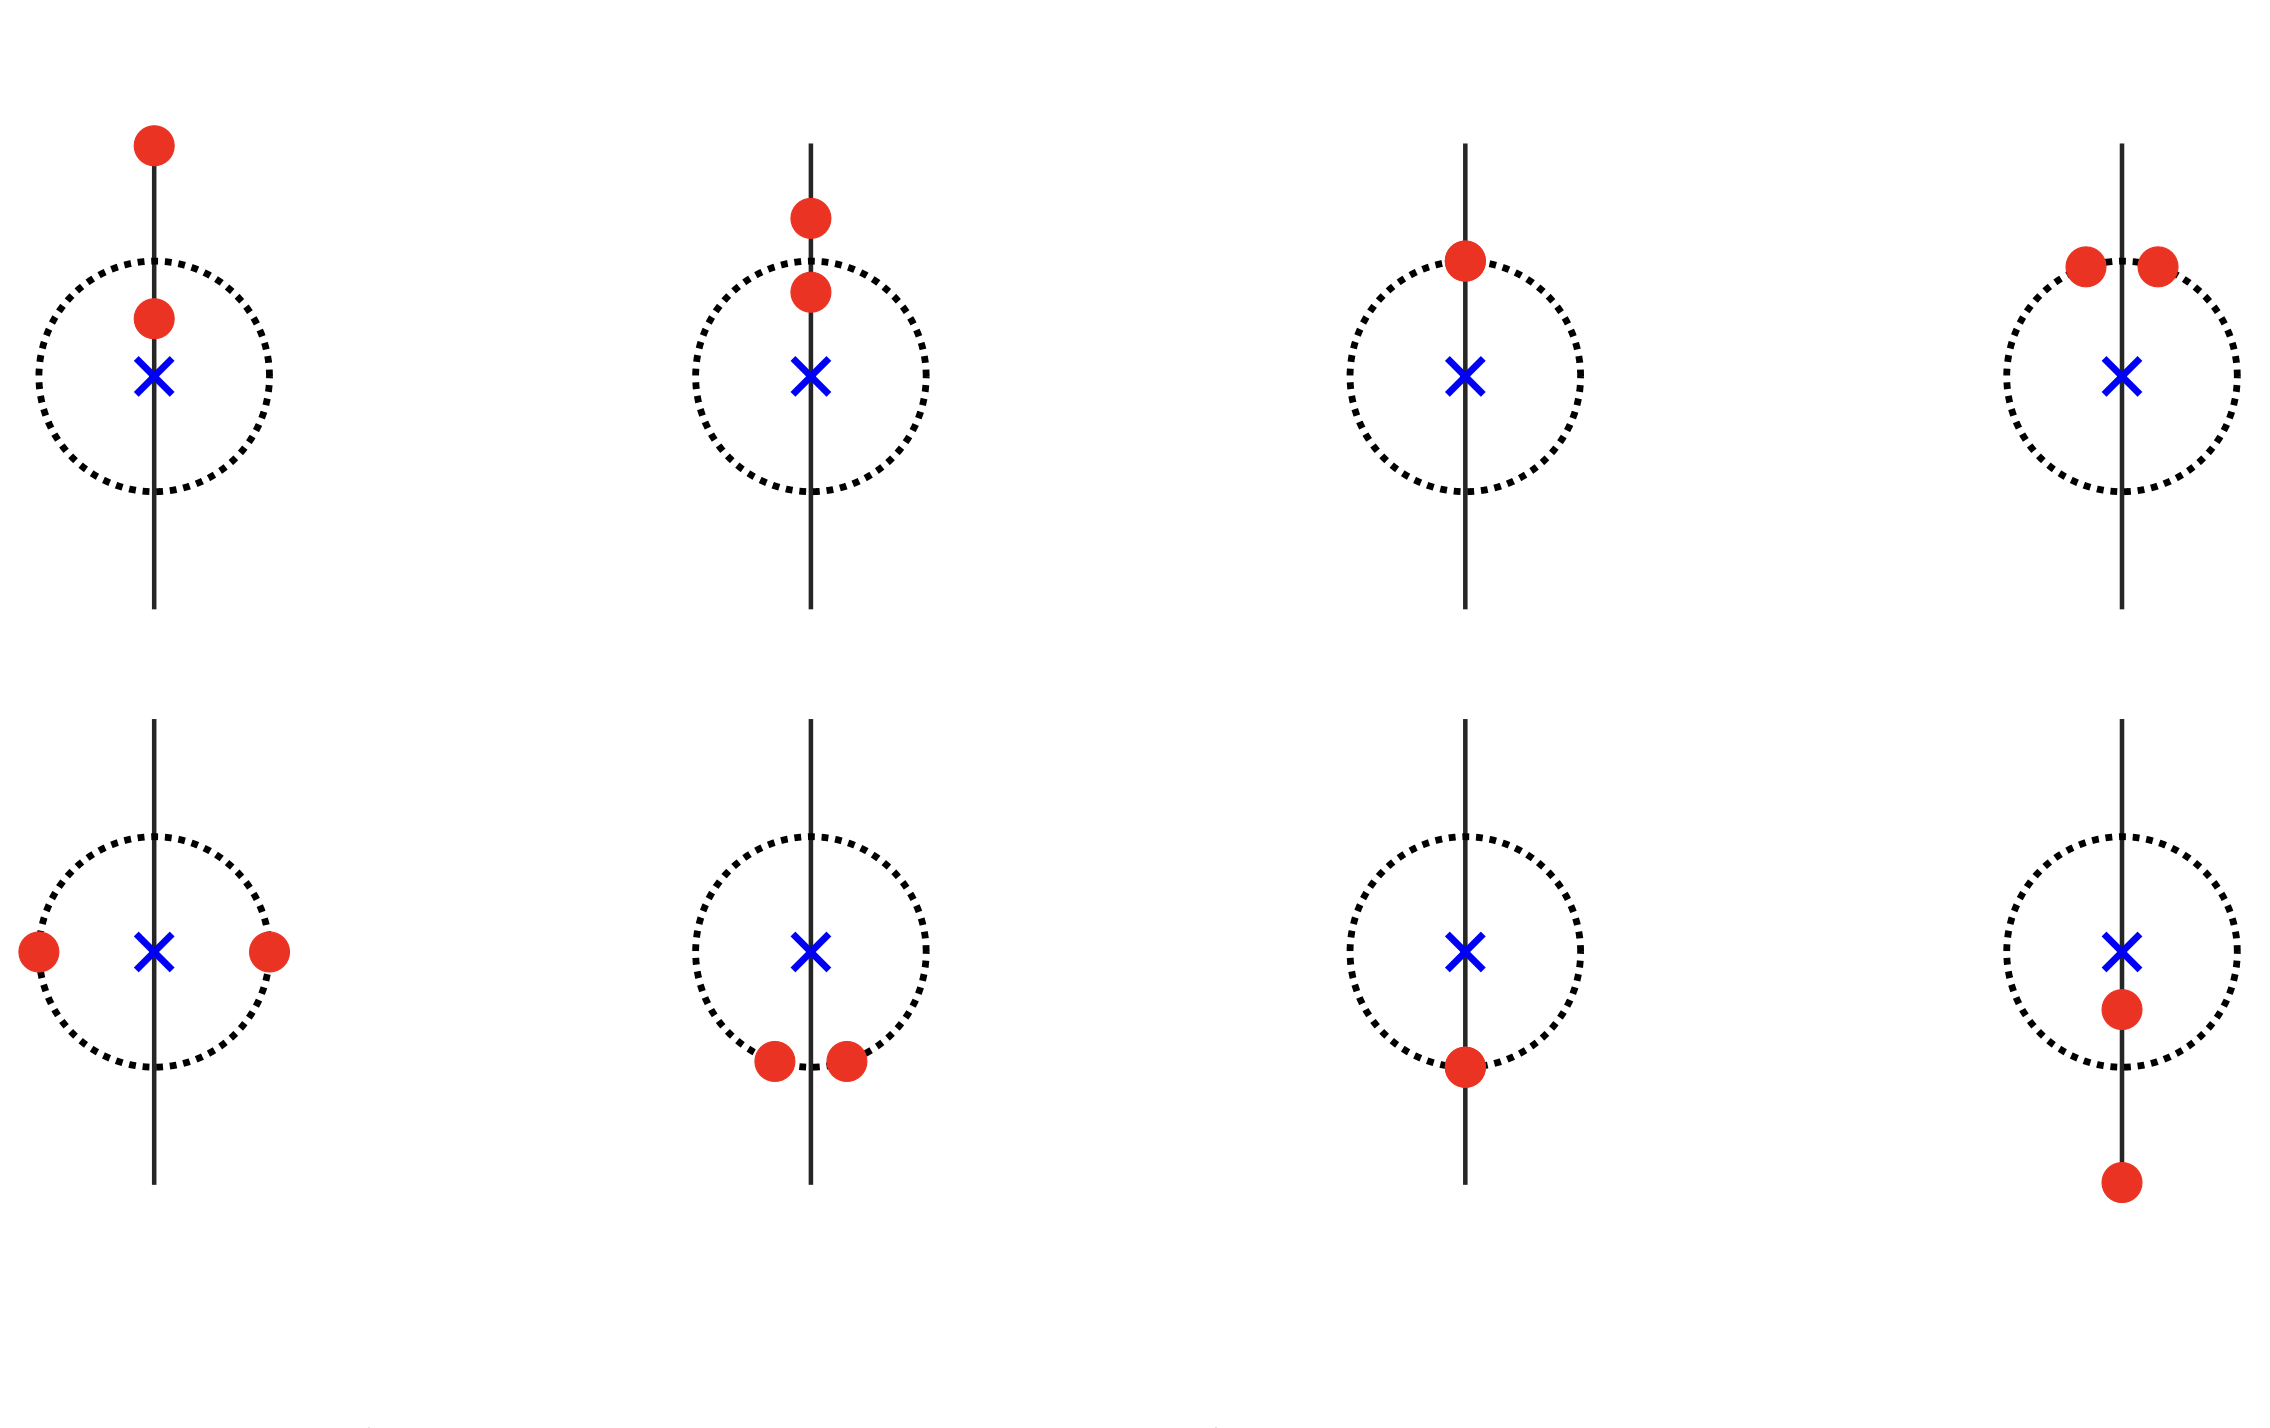
\includegraphics[width=9cm]{images/KreinBubbleCartoonSS2.png} & 
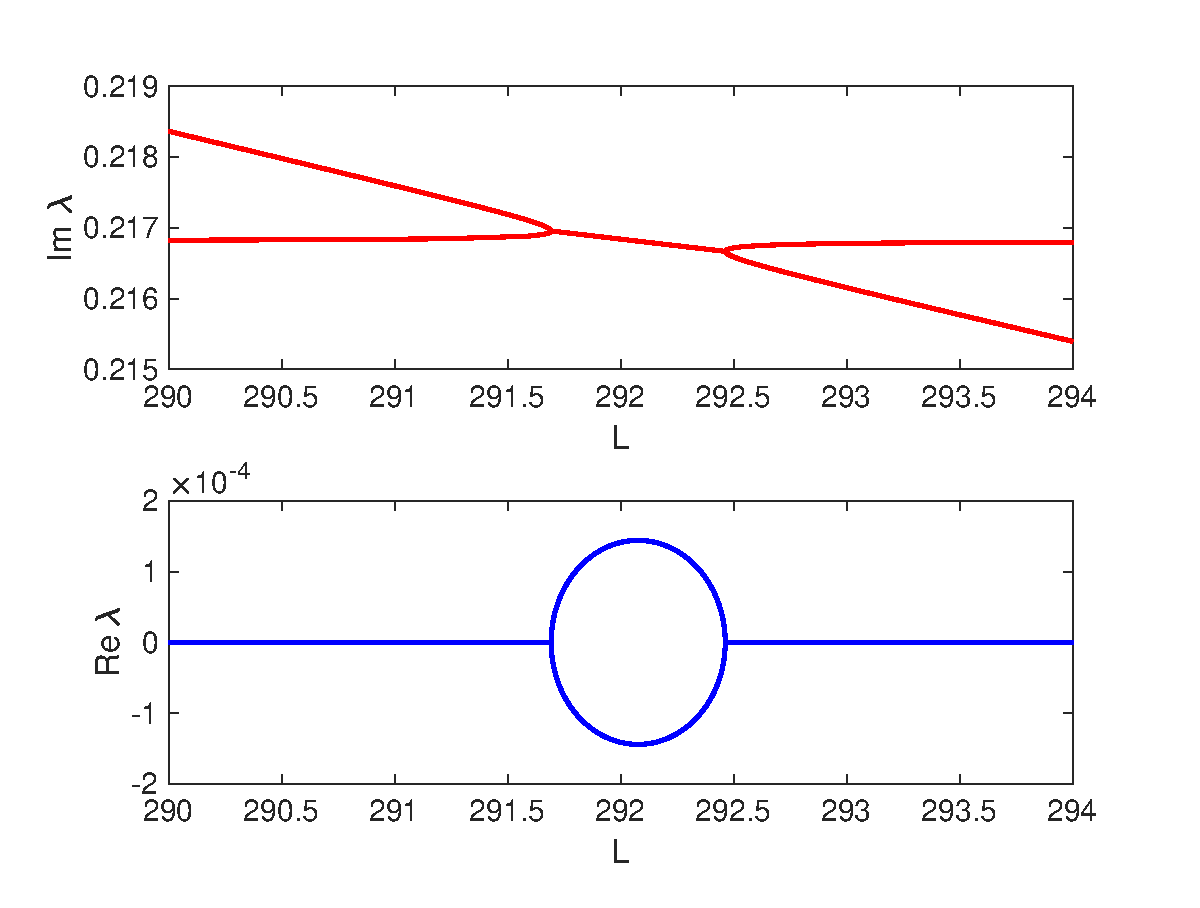
\includegraphics[width=8cm]{images/kreinbubble1.eps}
\end{tabular}
\end{center}
\caption{Krein instability bubble cartoon (left) and numerical simulation for KdV5 (right).}
\label{fig:kreinbubble1}
\end{figure}

\subsection*{Fourth order nonlinear Schr\"odinger equation}

The fourth-order nonlinear Schr{\"o}dinger equation (NLS4) 
\begin{align*}
    i u_t + \frac{\beta_4}{24}u_{xxxx} - \frac{\beta_2}{2}u_{xx} + \gamma |u|^2 u &= 0 
\end{align*}
is a variant of the nonlinear Schr{\"o}dinger equation which was introduced to account for the role of small fourth-order dispersion terms in the propagation of intense laser beams in a bulk medium with Kerr nonlinearity \cite{Karpman2000,Tam2020}. There is particular interest in the case where $\beta_2 = 0$, in which case the system exhibits pure quartic dispersion, since the corresponding solitary waves, known as pure quartic solitons, have been created experimentally \cite{Tam2019}. I prove that while multi-pulse solitary wave solutions exist, they are all unstable due to the presence of at least one eigenvalue with positive real part \cite[Theorems 1 and 2]{Parker2020NLS4}.

\subsection*{Other systems and future directions}

Other systems of interest include the discrete sine-Gordon equation, nonlocal lattice equations, and equations on higher dimensional lattices. The discrete sine-Gordon equation
\begin{align*}
	\frac{d^2}{dt^2}u_n &= d (\Delta_2 u)_n - \sin(u_n) && n \in \mathbb{Z}
\end{align*}
was introduced to describe the dynamics of crystal lattices, and has since been used in numerous applications, including a mechanical model for a chain of pendulums coupled with elastic springs, arrays of Josephson junctions, and DNA dynamics \cite{braun2004}. A particular class of coherent structures of interest in this system are kinks, which are exponentially localized stationary solutions connect adjacent minima of the potential $V(u) = \cos u$. In \cite{parkerSG}, I prove the existence of stationary multi-kink solutions as well as analyze their spectral stability. Another important class of coherent structures in this system are breathers, which are localized, oscillatory patterns. Future work involves using Lin's method to construct multi-site breathers by splicing together multiple, sequential copies of the primary breather and then analyzing their spectral stability.

One nonlocal version of DNLS \cite{Kirkpatrick2013} is
\begin{align*}
    i \frac{d}{dt} u_n = \frac{1}{h^{2s}} \sum_{m \neq n} \frac{u_m - u_n}{|m - n|^{1+2s}} + |u_n|^2 u_n && n \in \mathbb{Z},
\end{align*}
where $s > 0$ is a fixed parameter specifying the decay of the nonlocal interactions. In the continuum limit $h\rightarrow 0$, this equation converges to an NLS equation with fractional Laplacian \cite{Kirkpatrick2013}. Applications include a model for charge transport in DNA polymers. Future directions include studying solitary wave and multi-pulse solutions in this system, as well as whether the nonlocal interaction term permits other solutions which are not found in DNLS. A final, related area of interest is coherent structures in DNLS on the square integer lattice $\mathbb{Z}^2$, which could include nonlocal interactions in one or both directions. 

\section*{Coherent structures in optical lattices}

There has been much recent interest, both by experimental physicists and applied mathematicians, in the propagation dynamics of light pulses through arrays of optical fibers. One particular application is light transmission through multi-core optical fibers. In particular, optical transmission properties can be tuned by introducing a twist to the fiber bundle \cite{Longhi2016,CastroCastro2016,Parto2017} (\cref{fig:twist}).
\begin{figure}
\begin{center}
\begin{tabular}{cc}
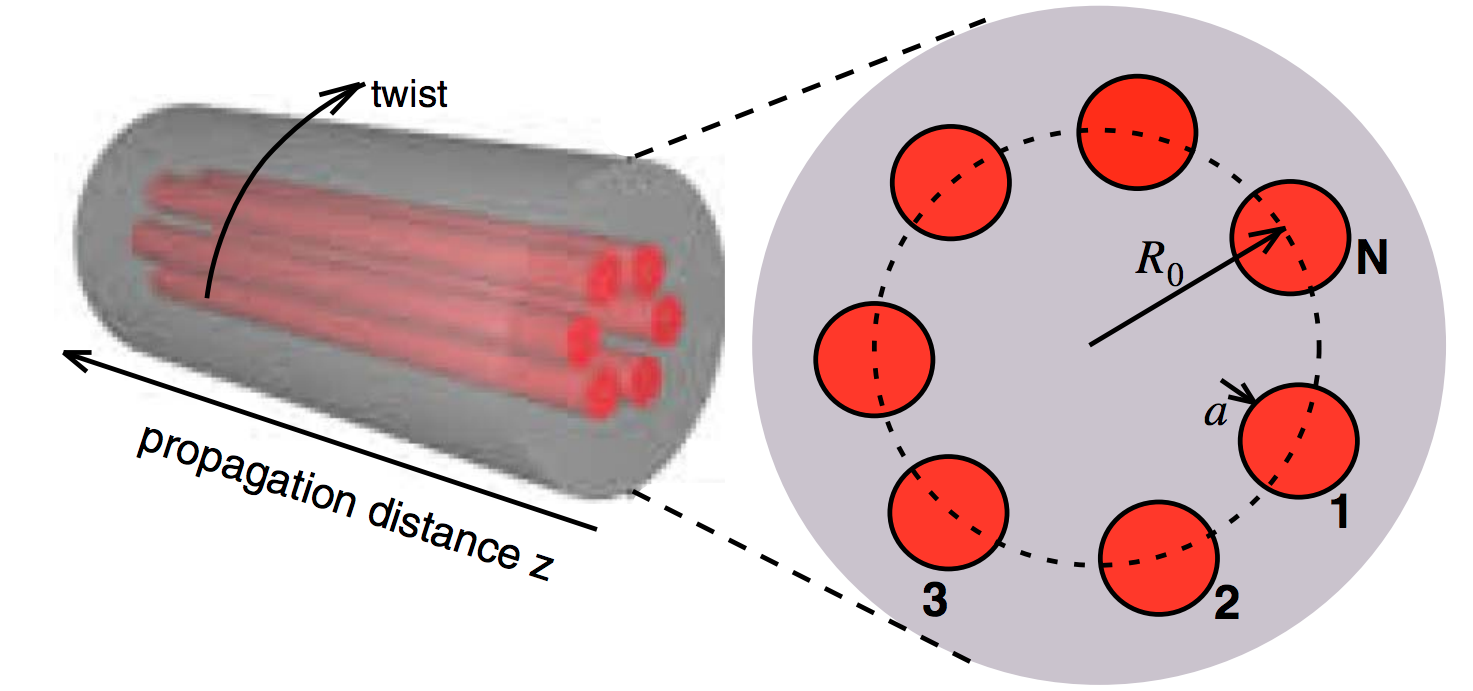
\includegraphics[width=7cm]{images/twist2.png} &
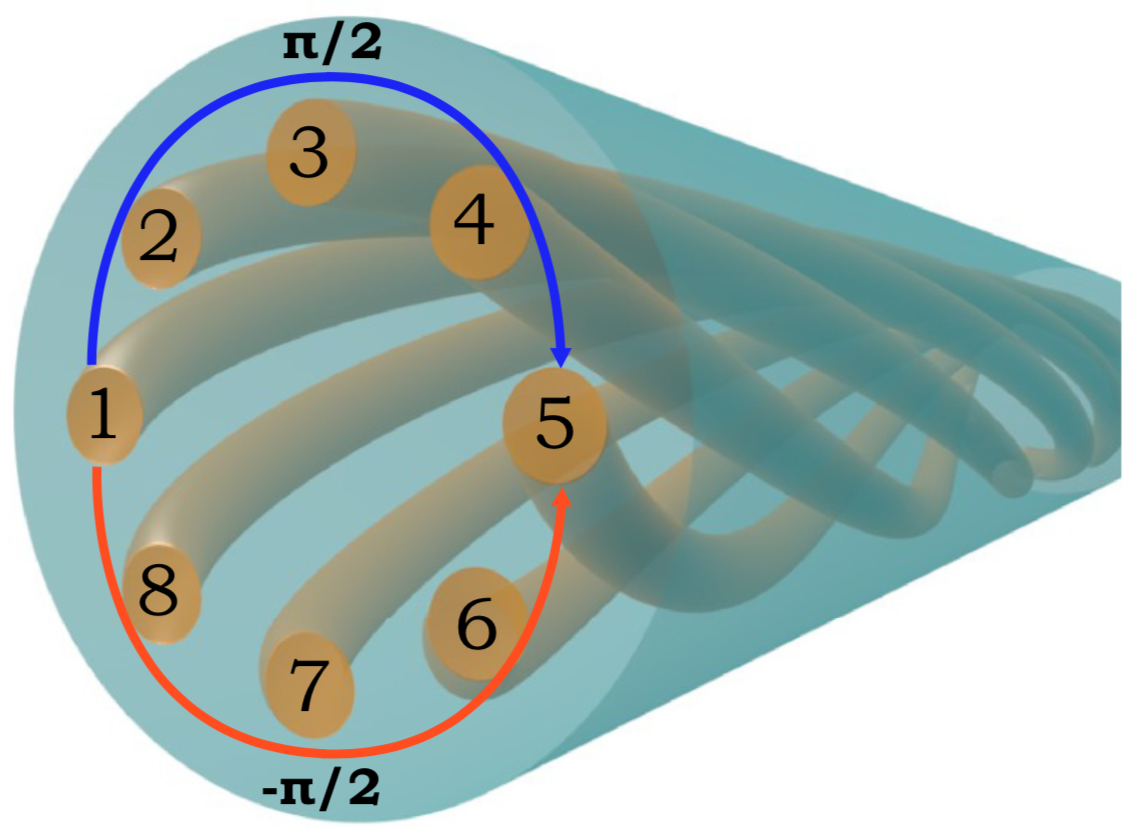
\includegraphics[width=4.25cm]{images/twistmulticore.png}
\end{tabular}
\end{center}
\caption{Circular multi-core fiber \cite{Longhi2016} (left) and twisted multi-core fiber with eight waveguides \cite{Parto2017} (right).}
\label{fig:twist}
\end{figure}
The propagation of light through a system of $N$ waveguides arranged in a circle can be described by the coupled mode equations
\begin{align*}
i \frac{d}{dz} c_n &= k \left(e^{-i\phi}c_{n+1} + e^{i\phi}c_{n-1}\right) + |c_n|^2 c_n &&  n = 1, \dots, N,
\end{align*}
where $z$ is the axis of propagation, $c_0 = c_{N}$ and $c_{N+1} = c_1$ due to the circular geometry, $k$ is the strength of the nearest-neighbor coupling, and $\phi$ is a parameter representing the twist of the fiber.  When the twist parameter $\phi$ and the number of fibers in the bundle $N$ are related by $\phi = \pi/N$, I prove that there is a stable standing wave solution of the form $c_n(z) = a_n e^{i \omega z}$ which has a ``dark node'' with no optical activity opposite a ``bright node'' of maximum intensity \cite{ParkerTwist} (\cref{fig:twistcn}). 
\begin{figure}
\begin{center}
\begin{tabular}{cc}
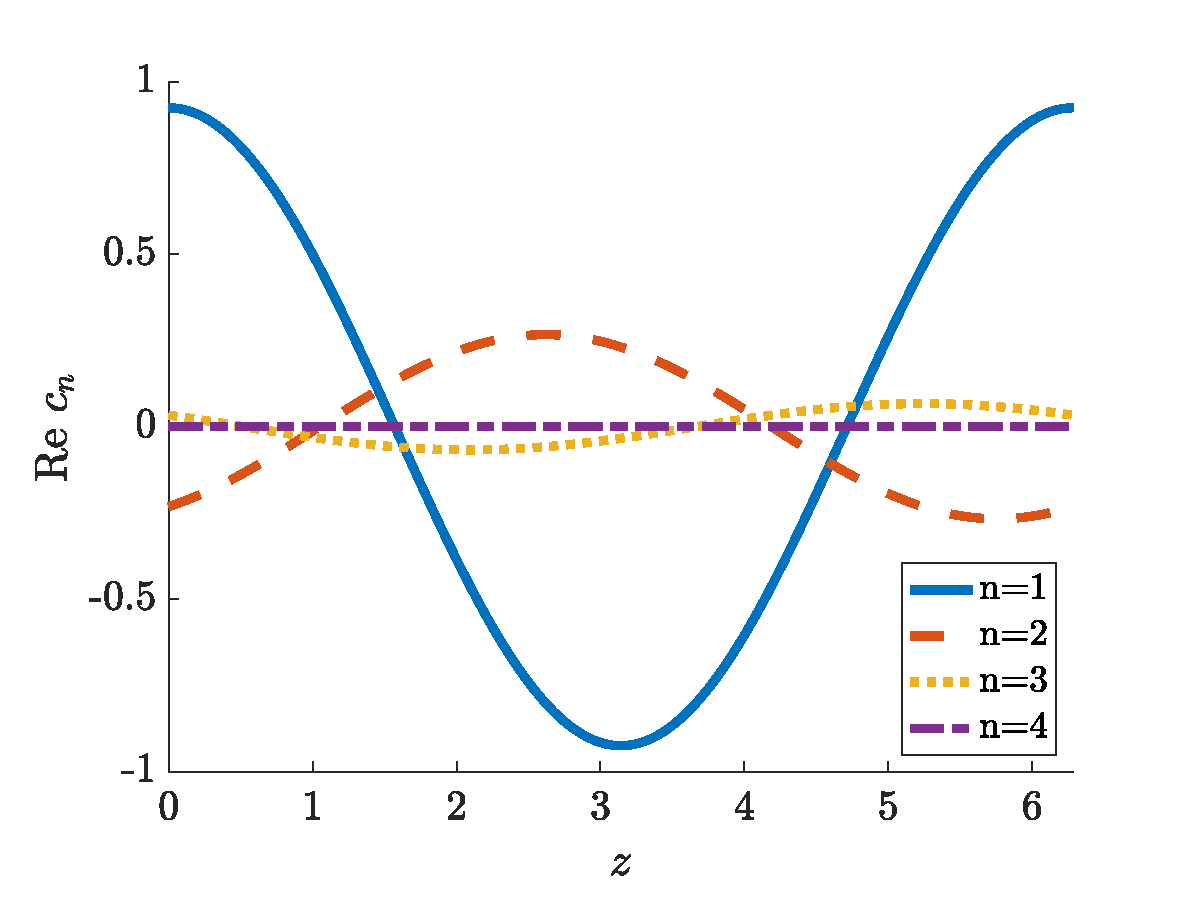
\includegraphics[width=8cm]{images/evenholestandingwave.eps} &
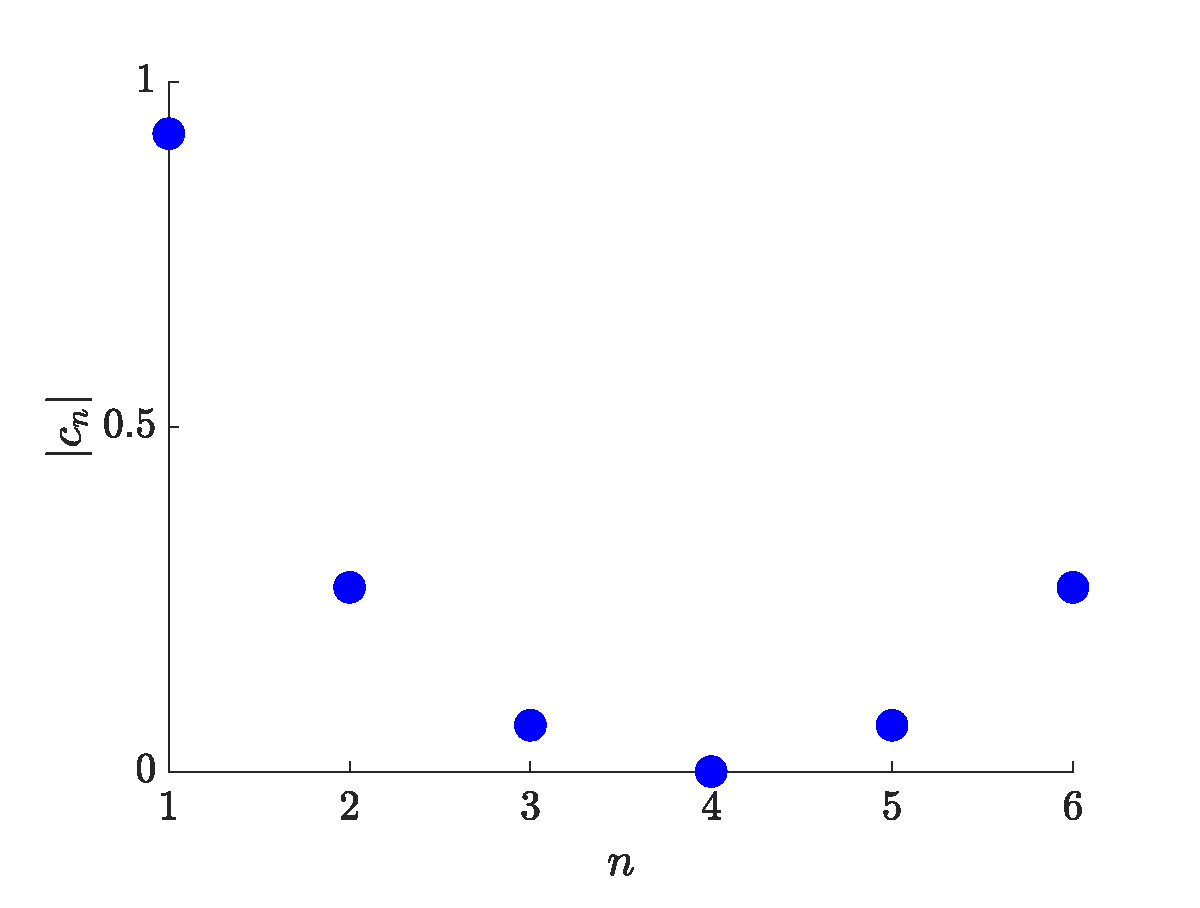
\includegraphics[width=8cm]{images/evenholeamps.eps}
\end{tabular}
\end{center}
\caption{Standing wave solution $c_n(z)$ for twisted multi-core fiber with $N = 6$ and $\phi = \pi/6$. Evolution of real part of solution for first four sites (left) and magnitude of solution at the sites (right). Site 1 has maximum intensity, and opposite site 4 has zero intensity.}
\label{fig:twistcn}
\end{figure}

Future research involves studying coherent structures in two-dimensional arrays of optical fibers and correlating the results from the mathematical models with experimental data. One example is a waveguide consisting of a square lattice of fibers in which there are periodic variations along the waveguide axis causing the nearest-neighbor coupling to vary periodically in $z$ \cite{Mukherjee2020}. In particular, for any $z$, a waveguide is only coupled to one of its four neighbors (\cref{fig:Rechtsman}, top). This configuration gives rise to periodic breather solutions in which the optical intensity is confined to a single square in the lattice but ``jumps'' around that square. No systematic mathematical study of the existence and stability of these solutions has been done to date. Other, more complicated arrangements of fibers which are of interest to experimentalists include concentric rings and honeycomb lattices \cite{Lumer2013}.

\begin{figure}
    \centering
    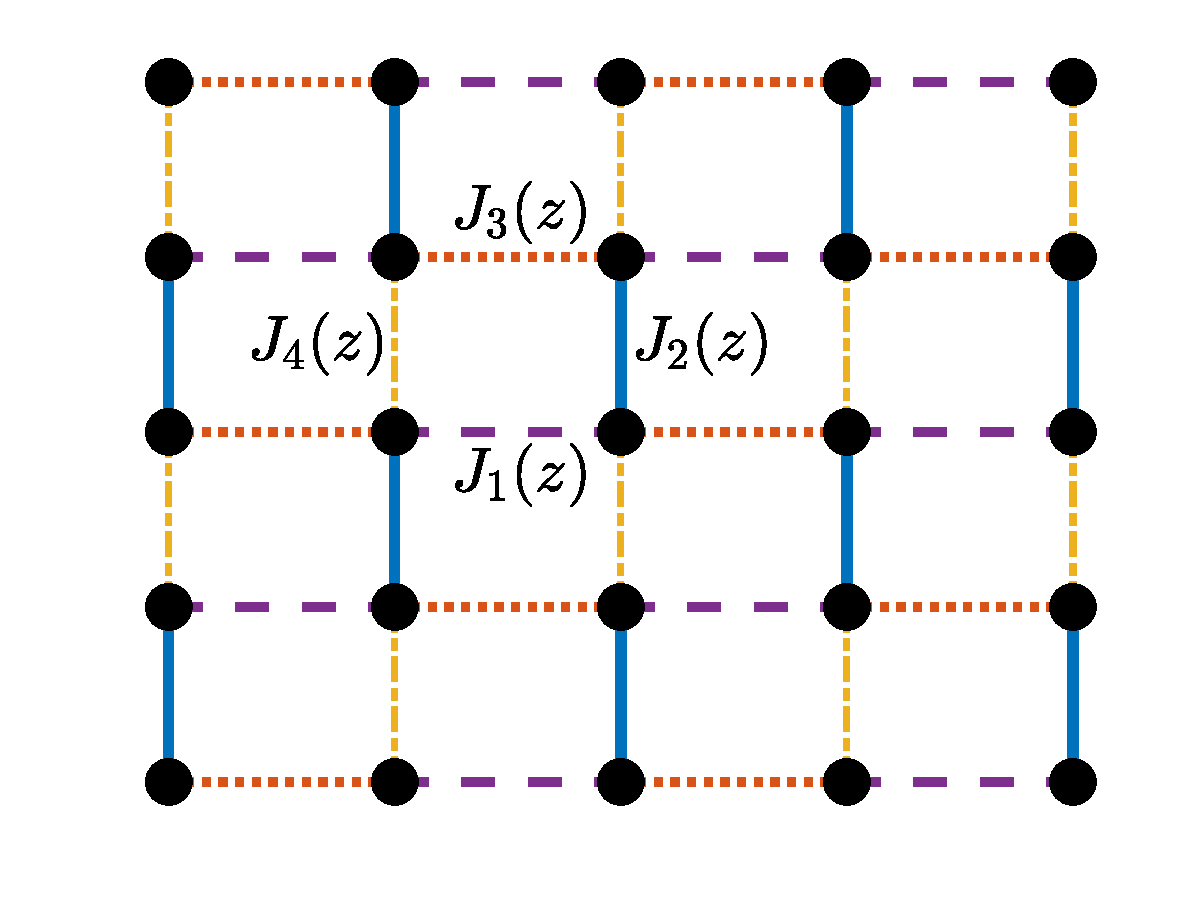
\includegraphics[width=7.8cm]{images/lattice.eps}
    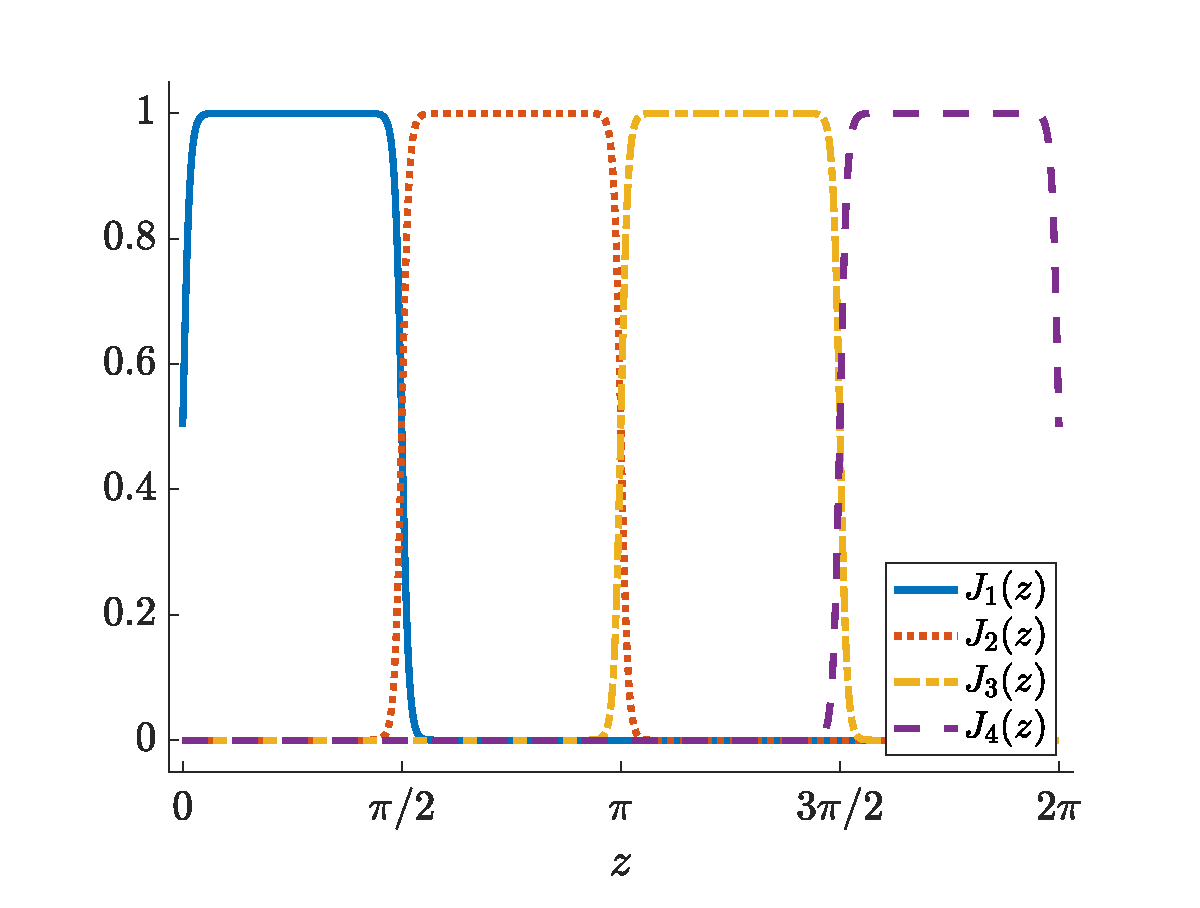
\includegraphics[width=7.8cm]{images/Jplot.eps}
    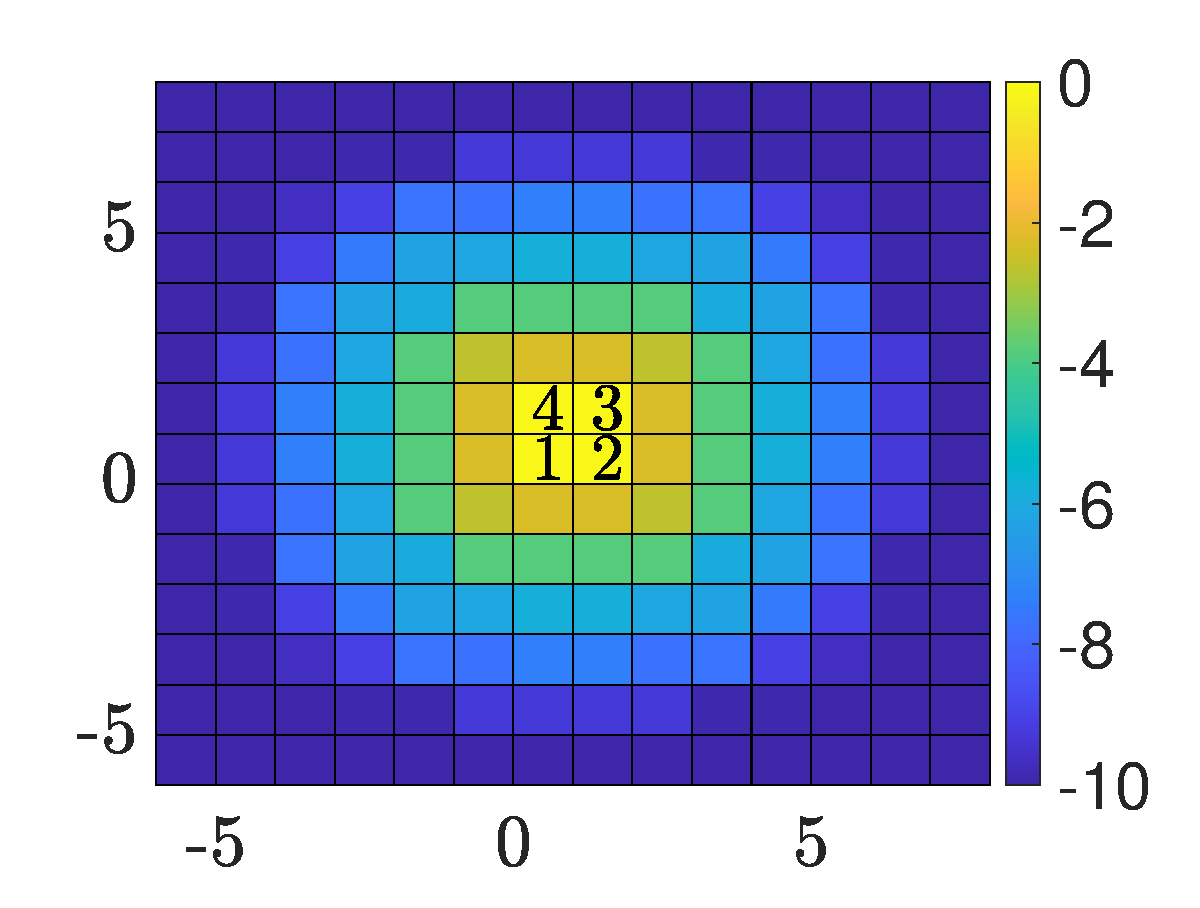
\includegraphics[width=7.8cm]{images/fundc1map.eps}
    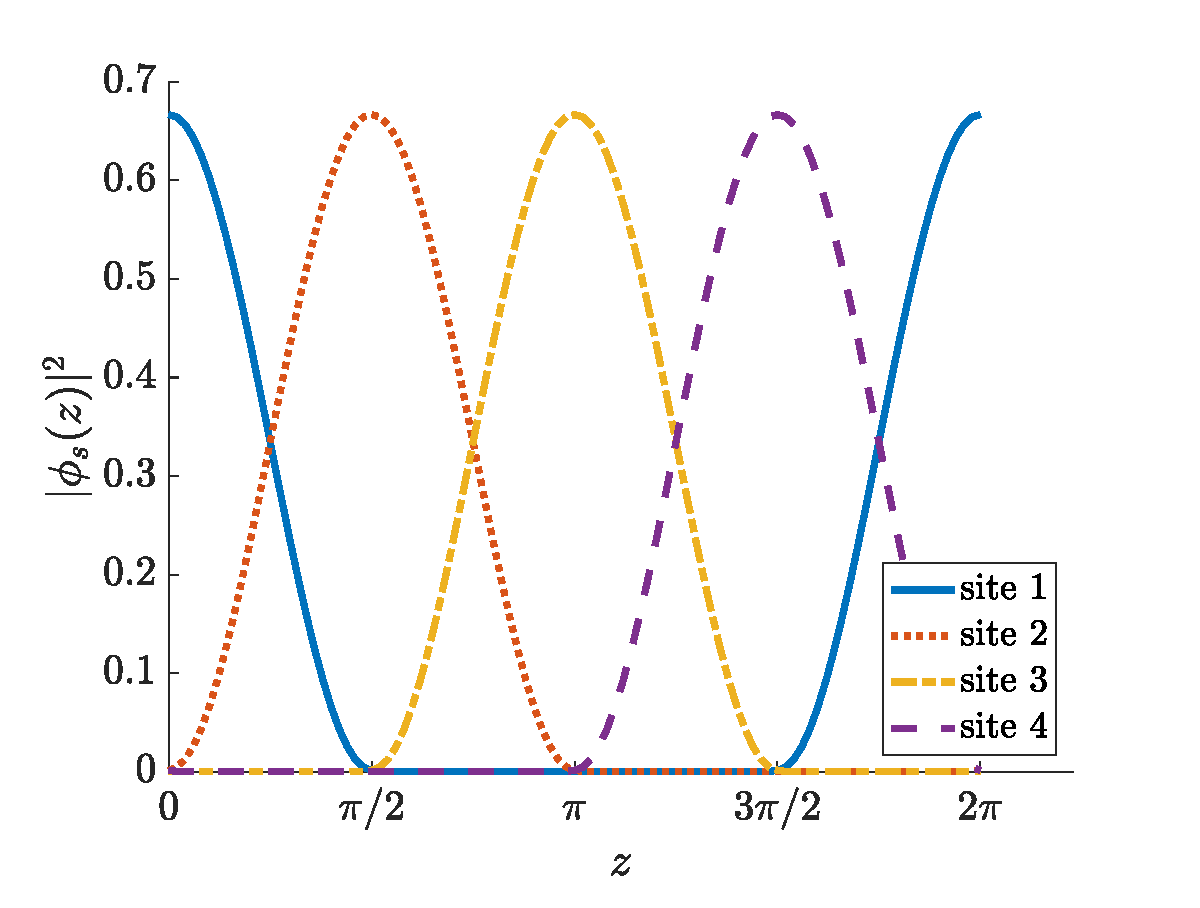
\includegraphics[width=7.8cm]{images/fundc1sol.eps}
    \caption{Cartoon of square lattice with $z$-dependent coupling (top left). The corresponding coupling functions (top right) cause each fiber to only interact with a single neighbor for any $z$. Bottom left is plot of log intensity of breather solution over one period, showing localization to a single unit square in lattice. Bottom right is square intensity of the breather solution on the unit square over one period.}
    \label{fig:Rechtsman}
\end{figure} 

\pagebreak
\bibliographystyle{siam}
\footnotesize{ \bibliography{researchstatement.bib} }

\end{document}
